%<<< TeX hoá bằng MyLT >>>
%<<< https://www.facebook.com/mylt2018 >>>

\documentclass[12pt,a4paper]{article}
\usepackage{amsmath,amssymb,fancyhdr}
\usepackage[top=1cm, bottom=1.5cm, left=1.5cm, right=1cm]{geometry}
\usepackage[dethi]{ex_test}
\usetikzlibrary{calc,patterns,intersections}
\newcommand{\heva}[1]{\left\{\begin{aligned}#1\end{aligned}\right.}
\pagestyle{fancy}
\fancyhf{}
\renewcommand{\headrulewidth}{0pt}
\renewcommand{\footrulewidth}{0pt}
\begin{document}
% \OPTN{kindTF=1t}
%Trái
\begin{minipage}[b]{4.5cm}
\centerline{\footnotesize\textbf{BỘ GIÁO DỤC VÀ ĐÀO TẠO}}
\centerline{\footnotesize\textbf{ĐỀ THI CHÍNH THỨC}}
\centerline{\footnotesize(\textit{Đề thi có \pageref{mylt}\ trang})}
\end{minipage}\hspace{1cm}
%Phải
\begin{minipage}[b]{12cm}
\centerline{\footnotesize\textbf{KỲ THI TỐT NGHIỆP TRUNG HỌC PHỔ THÔNG NĂM 2025}}
\centerline{\footnotesize\textbf{Môn thi: TOÁN}}
\centerline{\footnotesize\textit{Thời gian làm bài: 90\ phút, không kể thời gian phát đề}}
\end{minipage}\\
%Họ tên
\begin{minipage}[b]{10cm}
\vspace{6pt}\textbf{Họ và tên thí sinh: }{\tiny\dotfill}\\
\textbf{Số báo danh: }{\tiny\dotfill}
\end{minipage}\hfill
\begin{minipage}[b]{7.5cm}
\flushright\fbox{\bf Mã đề: 0105\quad \LaTeX\,hoá - MyLT}
\end{minipage}\hfill
%chân trang
\rfoot{Trang \thepage/\pageref{mylt} - Mã đề 0105}
\noindent\textbf{PHẦN I.} Thí sinh trả lời từ câu 1 đến câu 12. Mỗi câu hỏi thí sinh chỉ chọn một phương án.
\Opensolutionfile{ans}[ansMyLTTN]
\begin{ex}%Câu 1
Trong mặt phẳng với hệ tọa độ $O x y$, diện tích $S$ của hình phẳng giới hạn bởi đồ thị của hàm số $y=2x-3$, trục hoành và hai đường thẳng $x=1, x=2$ được xác định bằng công thức
\choice
{$S=\displaystyle\int\limits_1^2|2 x-3| d x$}
{$S=\pi \displaystyle\int\limits_1^2(2 x-3)^2 \mathrm{~d}x$}
{$S=\pi \displaystyle\int\limits_1^2|2 x-3| d x$}
{$S=\left|\displaystyle\int\limits_1^2(2 x-3) \mathrm{d}x\right|$}
\end{ex}

\begin{ex}%Câu 2
Nghiệm của phương trình $\log_3(2x-1)=2$ là
\choice
{$x=\dfrac{7}{2}$}
{$x=4$}
{$x=5$}
{$x=\dfrac{5}{2}$}
\end{ex}

\begin{ex}%Câu 3
Họ nguyên hàm của hàm số $f(x)=x^2$ là
\choice
{$3x^3+C$}
{$\dfrac{1}{2}x^3+C$}
{$2x^3+C$}
{$\dfrac{1}{3}x^3+C$}
\end{ex}

\begin{ex}%Câu 4
Một người chia thời lượng (đơn vị: giây) thực hiện các cuộc gọi điện thoại của mình trong một tuần thành sáu nhóm và lập bảng tần số ghép nhóm như sau.\\
\centerline{\begin{tabular}{|l|c|c|c|c|c|c|}
\hline Nhóm &{$[0; 40)$}&{$[40; 80)$}&{$[80; 120)$}&{$[120; 160)$}&{$[160; 200)$}&{$[200; 240)$}\\
\hline Tần số & 11 & 10 & 6 & 8 & 4 & 1 \\
\hline
\end{tabular}}\\
Tứ phân vị thứ ba $Q_3$ (đơn vị: giây) của mẫu số liệu ghép nhóm trên bằng
\choice
{135}
{130}
{145}
{140}
\end{ex}

\begin{ex}%Câu 5
Trong không gian với hệ tọa độ $Oxyz$, mặt phẳng đi qua điểm $A(2; 1;-4)$ nhận $\vec{n}=(3; 2;-1)$ làm một vectơ pháp tuyến có phương trình là
\choice
{$2(x+3)+(y+2)-4(z-1)=0$}
{$3(x-2)+2(y-1)-(z+4)=0$}
{$3(x+2)+2(y+1)-(z-4)=0$}
{$2(x-3)+(y-2)-4(z+1)=0$}
\end{ex}

\begin{ex}%Câu 6
\immini{
Cho hình lăng trụ $ABC.A^{\prime}B^{\prime}C^{\prime}$ (xem hình dưới). Phát biểu nào sau đây là \textbf{đúng}?
\choice
{$\overrightarrow{B A}+\overrightarrow{A^{\prime}C^{\prime}}=\overrightarrow{A^{\prime}A}$}
{$\overrightarrow{B A}+\overrightarrow{A^{\prime}C^{\prime}}=\overrightarrow{B C}$}
{$\overrightarrow{B A}+\overrightarrow{A^{\prime}C^{\prime}}=\overrightarrow{B C^{\prime}}$}
{$\overrightarrow{B A}+\overrightarrow{A^{\prime}C^{\prime}}=\overrightarrow{C^{\prime}B^{\prime}}$}
}{
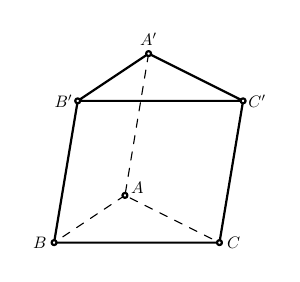
\begin{tikzpicture}[line join=round, line cap=round,thick,scale=0.6]
\coordinate (vtv) at (0.5,3);
\coordinate (A) at (0,0);
\coordinate (B) at (-1.5,-1);
\coordinate (C) at (2,-1);
\coordinate (A') at ($(A)+(vtv)$);
\coordinate (B') at ($(B)+(vtv)$);
\coordinate (C') at ($(C)+(vtv)$);
\draw(B')--(B)--(C)--(C')--(A')--(B')--(C');
\draw[dashed,thin](A')--(A)--(C) (A)--(B);
\foreach \i/\g in {A'/90,A/30,B/180,C/0,C'/0,B'/180}{\draw[fill=white](\i) circle (1.5pt) ($(\i)+(\g:3mm)$) node[scale=0.6]{$\i$};}
\end{tikzpicture}
}
\end{ex}

\begin{ex}%Câu 7
\immini{
Cho hàm số $y=\dfrac{ax+b}{cx+d}\,(ac \neq 0, ad-bc \neq 0)$ có đồ thị như hình dưới. Đường tiệm cận đứng của đồ thị hàm số đã cho có phương trình là
\choice
{$x=2$}
{$y=-1$}
{$y=2$}
{$x=-1$}
}{
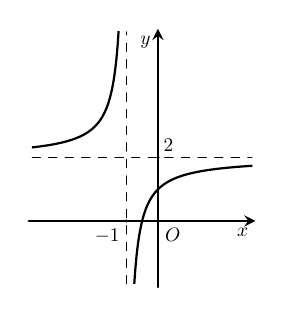
\begin{tikzpicture}[line join=round, line cap=round,>=stealth,thick,scale=0.4]
\tikzset{every node/.style={scale=0.7}}
\draw[->] (-4.1,0)--(3.1,0) node[below left] {$x$};
\draw[->] (0,-2.1)--(0,6.1) node[below left] {$y$};
\draw (0,0) node [below right] {$O$};
\draw[thin] (-1,1pt)--(-1,-1pt) node [below left] {$-1$};
\draw[thin] (1pt,2)--(-1pt,2) node [above right] {$2$};
\draw[dashed,thin] (-0.99,-2)--(-0.99,6);
\begin{scope}
\clip (-4,-2) rectangle (3,6);
\draw[samples=200,domain=-4:-1.01,smooth,variable=\x] plot (\x,{(2*(\x)+1)/(1*(\x)+1)});
\draw[samples=200,domain=-0.99:3,smooth,variable=\x] plot (\x,{(2*(\x)+1)/(1*(\x)+1)});
\draw[dashed,thin] (-4,2/1)--(3,2/1);
\end{scope}
\end{tikzpicture}
}
\end{ex}

\begin{ex}%Câu 8
Cho hình chóp $S.ABC$ có $SA$ vuông góc với mặt phẳng $(ABC)$, tam giác $ABC$ vuông tại $A$ và $SA=3, AB=4, AC=5$. Thể tích của khối chóp $S.ABC$ bằng
\choice
{$20$}
{$60$}
{$30$}
{$10$}
\end{ex}

\begin{ex}%Câu 9
Cho cấp số cộng $\left(u_n\right)$ có $u_1=4$ và công sai $d=-3$. Giá trị của $u_5$ bằng
\choice
{$-8$}
{$19$}
{$16$}
{$-11$}
\end{ex}

\begin{ex}%Câu 10
\immini{
Cho hình hộp $ABCD.A^{\prime}B^{\prime}C^{\prime}D^{\prime}$ (xem hình dưới). Đường thẳng $AB$ song song với mặt phẳng nào sau đây?
\choice
{$\left(AA^{\prime}D^{\prime}D\right)$}
{$\left(CC^{\prime}A^{\prime}A\right)$}
{$\left(BB^{\prime}C^{\prime}C\right)$}
{$\left(A^{\prime}B^{\prime}C^{\prime}D^{\prime}\right)$}
}{
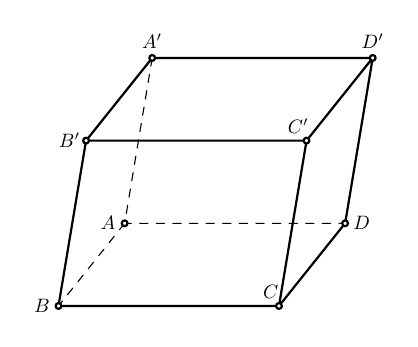
\begin{tikzpicture}[line join=round, line cap=round,thick,scale=0.7]
\coordinate (vtv) at (0.5,3);
\coordinate (A) at (0,0);
\coordinate (B) at (-1.2,-1.5);
\coordinate (D) at (4,0);
\coordinate (C) at ($(B)+(D)-(A)$);
\coordinate (A') at ($(A)+(vtv)$);
\coordinate (B') at ($(B)+(vtv)$);
\coordinate (C') at ($(C)+(vtv)$);
\coordinate (D') at ($(D)+(vtv)$);
\draw(B')--(B)--(C)--(C')--(B')--(A')--(D')--(C') (C)--(D)--(D');
\draw[dashed,thin](A')--(A)--(D) (A)--(B);
\foreach \i/\g in {A'/90,A/180,B/180,C/120,D/0,B'/180,D'/90,C'/120}{\draw[fill=white](\i) circle (1.5pt) ($(\i)+(\g:3mm)$) node[scale=0.7]{$\i$};}
\end{tikzpicture}
}
\end{ex}

\begin{ex}%Câu 11
Tập nghiệm của phương trình $\sin x=0$ là
\choice
{$S=\{k2\pi \mid k \in \mathbb{Z}\}$}
{$S=\left\{\left.\dfrac{\pi}{2}+k\pi\right\rvert\, k \in \mathbb{Z}\right\}$}
{$S=\{k\pi \mid k \in \mathbb{Z}\}$}
{$S=\left\{\left.\dfrac{\pi}{2}+k2\pi \right\rvert\, k \in \mathbb{Z}\right\}$}
\end{ex}

\begin{ex}%Câu 12
Trong không gian với hệ tọa độ $Oxyz$, cho đường thẳng $(d): \dfrac{x-3}{4}=\dfrac{y+2}{-5}=\dfrac{z-1}{2}$. Vectơ nào sau đây là một vectơ chỉ phương của đường thẳng $(d)$?
\choice
{$\overrightarrow{v_2}=(4;-5; 2)$}
{$\overrightarrow{v_3}=(4; 5; 2)$}
{$\overrightarrow{v_1}=(3;-2; 1)$}
{$\overrightarrow{v_4}=(3; 2; 1)$}
\end{ex}
\Closesolutionfile{ans}

\noindent\textbf{PHẦN II.} Thí sinh trả lời từ câu 1 đến câu 4. Mỗi ý \textbf{a), b), c), d)} ở mỗi câu hỏi, thí sinh chọn đúng hoặc sai.
\setcounter{ex}{0}
\Opensolutionfile{ans}[ansMyLTTF]
\begin{ex}%Câu 13
Mô hình toán học sau đây được sử dụng trong quan sát chuyển động của một vật. Trong không gian cho hệ tọa độ $Oxyz$ có $\vec{i}, \vec{j}, \vec{k}$ lần lượt là các vectơ đơn vị trên các trục $Ox, Oy, Oz$ và độ dài của mỗi vectơ đơn vị đó bằng $1$ mét. Cho hai điểm $A$ và $B$, trong đó điểm $A$ có tọa độ là $(5; 5; 0)$. Một vật (coi như là một hạt) chuyển động thẳng với tốc độ phụ thuộc thời gian $t$ (giây) theo công thức $v(t)=\beta t+300$ (m/giây), trong đó $\beta$ là hằng số dương và $0 \leq t \leq 6$. Ở thời điểm ban đầu $(t=0)$, vật đi qua $A$ với tốc độ $300$ m/giây và hướng tới $B$. Sau $2$ giây kể từ thời điểm ban đầu, vật đi được quãng đường 604 m . Gọi $\vec{u}=(a; b; c)$ là vectơ cùng hướng với vectơ $\overrightarrow{AB}$. Biết rằng $|\vec{u}|=1$ và góc giữa vectơ $\vec{u}$ lần lượt với các vectơ $\vec{i}, \vec{j}, \vec{k}$ có số đo tương ứng bằng $60^{\circ}, 60^{\circ}, 45^{\circ}$.
\choiceTF
{$a=\cos 60^{\circ}$}
{Phương trình đường thẳng $AB$ là $\dfrac{x-5}{1}=\dfrac{y-5}{1}=\dfrac{z}{2}$}
{$\beta=2$}
{Giả sử sau $5$ giây kể từ thời điểm ban đầu, vật đến điểm $B\left(x_B; y_B; z_B\right)$. Khi đó $x_B>768$}
\end{ex}

\begin{ex}%Câu 14
Đối với ngành nuôi trồng thủy sản, việc kiểm soát lượng thuốc tồn đư trong nước là một nhiệm vụ quan trọng nhằm đáp ứng các tiêu chuẩn an toàn về môi trường. Khi nghiên cứu một loại thuốc trị bệnh trong nuôi trồng thủy sản, người ta sử dụng thuốc đó một lần và theo dõi nồng độ thuốc tồn dư trong nước kể từ lúc sử dụng thuốc. Kết quả cho thấy nồng độ thuốc $y(t)$ (đơn vị: mg/lít) tồn dư trong nước tại thời điểm $t$ ngày $(t \geq 0)$ kể từ lúc sử dụng thuốc, thỏa mãn $y(t)>0$ và $y^{\prime}(t)=k .y(t)(t \geq 0)$, trong đó $k$ là hằng số khác không. Đo nồng độ thuốc tồn dư trong nước tại các thời điểm $t=6$ (ngày); $t=12$ (ngày) nhận được kết quả lần lượt là $2$ mg/lít; $1$ mg/lít. Cho biết $y(t)=e^{g(t)}(t \geq 0)$.
\choiceTF
{$g(t)=k t+C\,(t \geq 0)$ với $C$ là một hằng số xác định}
{$k=\dfrac{\ln 2}{6}$}
{$C=2 \ln 2$}
{Nồng độ thuốc tồn dư trong nước tại thời điểm $t=25$ (ngày) kể từ lúc sử dụng thuốc lớn hơn $0,25$ mg/lít}
\end{ex}

\begin{ex}%Câu 15
Một phần mềm nhận dạng tin nhắn quảng cáo trên điện thoại bằng cách dựa theo từ khóa để đánh dấu một số tin nhắn được gửi đến. Qua một thời gian dài sử dụng, người ta thấy rằng trong số tất cả các tin nhắn gửi đến, có $15 \%$ số tin nhắn bị đánh dấu. Trong số các tin nhắn bị đánh dấu, có $10 \%$ số tin nhắn không phải là quảng cáo. Trong số các tin nhắn không bị đánh dấu, có $5 \%$ số tin nhắn là quảng cáo.
Chọn ngẫu nhiên một tin nhắn được gửi đến điện thoại.
\choiceTF
{Xác suất để tin nhắn đó không bị đánh dấu bằng $0,85$}
{Xác suất để tin nhắn đó không phải là quảng cáo, biết rằng nó không bị đánh dấu, bằng $0,95$}
{Xác suất để tin nhắn đó không phải là quảng cáo bằng $0,85$}
{Xác suất để tin nhắn đó không bị đánh dấu, biết rằng nó không phải là quảng cáo, lớn hơn $0,95$}
\end{ex}

\begin{ex}%Câu 16
Cho hàm số $f(x)=x^3-12x-8$.
\choiceTF
{Hàm số đã cho có đạo hàm là $f^{\prime}(x)=3x^2-12$}
{Phương trình $f^{\prime}(x)=0$ có tập nghiệm là $S=\{2\}$}
{$f(2)=24$}
{Giá trị lớn nhất của hàm số $f(x)$ trên đoạn $[-3; 3]$ bằng 24}
\end{ex}
\Closesolutionfile{ans}

\noindent\textbf{PHẦN III.} Thí sinh trả lời từ câu 1 đến câu 6.
\setcounter{ex}{0}
\Opensolutionfile{ans}[ansMyLTSA]
\begin{ex}%Câu 17
\immini{
Bạn Nam tham gia cuộc thi giải một mật thư. Theo quy tắc của cuộc thi, người chơi cần chọn ra sáu số từ tập $S=\{11; 12; 13; 14; 15; 16; 17; 18; 19\}$ và xếp mỗi số vào đúng một vị trí trong sáu vị trí $A, B, C, M, N, P$ như hình bên sao cho mỗi vị trí chỉ được xếp một số. Mật thư sẽ được giải nếu các bộ ba số xuất hiện ở những bộ ba vị trí $(A, M, B);(B, N, C);(C, P, A)$ tạo thành các cấp số cộng theo thứ tự đó. Bạn Nam chọn ngẫu nhiên $6$ số trong tập $S$ và xếp ngẫu nhiên vào các vị trí được yêu cầu. Gọi xác suất để bạn Nam giải được mật thư ở lần chọn và xếp đó là $a$. Giá trị của $\dfrac{1}{a}$ bằng bao nhiêu?
}{
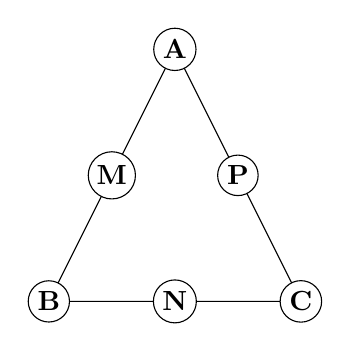
\begin{tikzpicture}[scale=1.6, every node/.style={circle, draw, inner sep=1.5pt, fill=white, font=\bfseries}]
    \coordinate (A) at (0,2);
    \coordinate (B) at (-1,0);
    \coordinate (C) at (1,0);
    \coordinate (M) at ($(A)!0.5!(B)$);
    \coordinate (N) at ($(B)!0.5!(C)$);
    \coordinate (P) at ($(A)!0.5!(C)$);
    \draw (A)--(M)--(B)--(N)--(C) --(P)--cycle;
    \node at (A) {A};
    \node at (B) {B};
    \node at (C) {C};
    \node at (M) {M};
    \node at (N) {N};
    \node at (P) {P};
\end{tikzpicture}
}
\end{ex}

\begin{ex}%Câu 18
Nếu một doanh nghiệp sản xuất $x$ sản phẩm trong một tháng $\left(x \in \mathbb{N}^*; 1 \leq x \leq 4500\right)$ thì doanh thu nhận được khi bán hết số sản phẩm đó là $F(x)=-0,01x^2+300x$ (nghìn đồng), trong khi chi phí sản xuất bình quân cho mỗi sản phẩm là $G(x)=\dfrac{30000}{x}+200$ (nghìn đồng). Giả sử số sản phẩm sản xuât ra luôn được bán hết. Trong một tháng, doanh nghiệp đó cần sản xuất ít nhất bao nhiêu sản phẩm để lợi nhuận thu được lớn hơn $100$ triệu đồng?
\end{ex}

\begin{ex}%Câu 19
Cho hình chóp $S.ABCD$ có đáy $ABCD$ là hình thoi với $\widehat{ABC}=60^{\circ}$ và $AB=2$. Biết rằng hình chiếu vuông góc của $S$ trên mặt phẳng $(ABCD)$ là trọng tâm $H$ của tam giác $ABC$ và $SH=\sqrt{3}$. Khoảng cách giữa hai đường thẳng $AC$ và $SD$ bằng bao nhiêu (\textit{không làm tròn kết quả các phép tính trung gian, chi làm tròn kết quả cuối cùng đến hàng phần trăm})?
\end{ex}

\begin{ex}%Câu 20
Để gây quỹ từ thiện, câu lạc bộ thiện nguyện của một trường THPT tổ chức hoạt động bán hàng với hai mặt hàng là nước chanh và khoai chiên. Câu lạc bộ thiết kế hai thực đơn. Thực đơn 1 có giá $30$ nghìn đồng, bao gồm hai cốc nước chanh và một túi khoai chiên. Thực đơn $2$ có giá $50$ nghìn đồng, bao gồm ba cốc nước chanh và hai túi khoai chiên. Biết rằng câu lạc bộ chỉ làm được không quá $165$ cốc nước chanh và $100$ túi khoai chiên. Số tiền lớn nhất mà câu lạc bộ có thể nhận được sau khi bán hết hàng bằng bao nhiêu nghìn đồng?
\end{ex}

\begin{ex}%Câu 21
Có $4$ ngăn (trong một giá để sách) được đánh số thứ tự $1,2,3,4$ và bảy quyển sách khác nhau. Bạn An xếp hết $7$ quyển sách nói trên vào $4$ ngăn đó sao cho mỗi ngăn có ít nhất một quyển sách và các quyển sách được xếp thẳng đứng thành một hàng ngang với gáy sách quay ra ngoài ở mỗi ngăn. Khi đã xếp xong $7$ quyển sách, hai cách xếp của bạn An được gọi là giống nhau nếu chúng thỏa mãn đồng thời hai điều kiện sau đây:\\
+ Với từng ngăn, số lượng quyển sách ở ngăn đó là như nhau trong cả hai cách xếp;\\
+ Với từng ngăn, thứ tự từ trái sang phải của các quyển sách được xếp là như nhau trong cả hai cách xếp.\\
Gọi $T$ là số cách xếp đôi một khác nhau của bạn An. Giá trị của $\dfrac{T}{100}$ bằng bao nhiêu?
\end{ex}

\begin{ex}%Câu 22
Để đặt được một vật trang trí trên mặt bàn, người ta thiết kế một chân đế như sau. Lấy một khối gỗ có dạng khối chóp cụt tứ giác đều với độ dài hai cạnh đáy lần lượt bằng $7,4 \mathrm{~cm}$ và $10,4 \mathrm{~cm}$, bề dày của khối gỗ bằng $1,5 \mathrm{~cm}$. Sau đó khoét bỏ đi một phần của khối gỗ sao cho phần đó có dạng vật thể $H$, ở đó $H$ nhận được bằng cách cắt khối cầu bán kính $5,8 \mathrm{~cm}$ bởi một mặt phẳng cắt mà mặt cắt là hình tròn bán kính $3,5 \mathrm{~cm}$ (xem hình dưới).\\
\centerline{
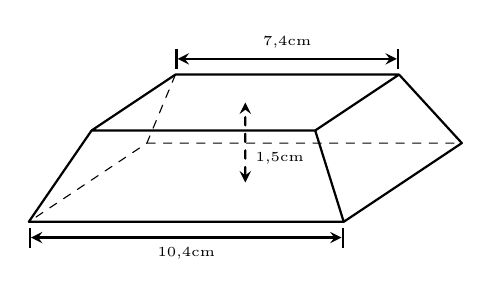
\begin{tikzpicture}[line join=round, line cap=round,>=stealth,thick]
	% Hình trái
	\coordinate (A) at (0,0);
	\coordinate (B) at (-1.5,-1);
	\coordinate (D) at (4,0);
	\coordinate (C) at ($(B)+(D)-(A)$);
	\coordinate (O) at ($(A)!0.5!(C)$);
	\coordinate (I) at ($(O)+(0,3.5)$);
	\coordinate (A') at ([scale around={0.71:(I)}] A);
	\coordinate (B') at ([scale around={0.71:(I)}] B);
	\coordinate (C') at ([scale around={0.71:(I)}] C);
	\coordinate (D') at ([scale around={0.71:(I)}] D);
	\coordinate (O') at ($(A')!0.5!(C')$);
	\draw(B)--(C)--(D)--(D')--(C')--(B')--(A')--(D') (C)--(C') (B)--(B');
	\draw[dashed,thin](A')--(A)--(B) (A)--(D);
	\draw[dashed,<->](O)--(O')node[right,pos=0.3]{\tiny 1,5cm};
	\coordinate (vt) at (0,0.2);
	\coordinate (A1) at ($(A')+(vt)$);
	\coordinate (D1) at ($(D')+(vt)$);
	\draw[|<->|](A1)--(D1)node[above,sloped,pos=0.5]{\tiny 7,4cm};
	\coordinate (vt1) at (0,0.1);
	\coordinate (B1) at ($(B)-(vt)$);
	\coordinate (C1) at ($(C)-(vt)$);
	\draw[|<->|](B1)--(C1)node[below,sloped,pos=0.5]{\tiny 10,4cm};
\end{tikzpicture}\qquad

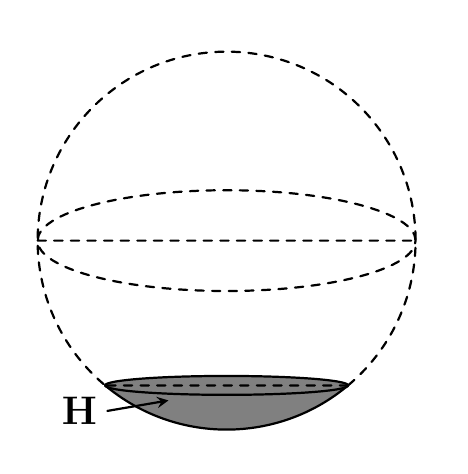
\begin{tikzpicture}[line join=round, line cap=round,>=stealth,thick,scale=0.8]
	% Hình giữa
	\def\bk{3}
	\def\bkba{0.15}
	\def\bkbb{0.8}
	\def\ga{-50}
	\def\gb{180-\ga}
	\def\gc{0-\gb}
	\coordinate (O) at (0,0);
	\coordinate (M) at ($(O) + (\ga:\bk)$);
	\coordinate (N) at ($(O) + (\gb:\bk)$);
	\coordinate (I) at ($(M)!0.5!(N)$);
	\draw[name path=c1,dashed] (M) arc (\ga:\gb:\bk);
	\path let \p1=(I),\p2=(M),\n1={scalar(veclen(\x2-\x1,\y2-\y1)/1cm)} in \pgfextra{\xdef\bke{\n1}};
	\fill[gray](M) arc (\ga:\gc:\bk)--(N) arc (180:0:\bke cm and \bkba cm)--cycle;
	\draw[name path=c1] (M) arc (\ga:\gc:\bk);
	\draw[name path=ne1] (M) arc (0:180:\bke cm and \bkba cm);
	\draw[name path=ne1] (M) arc (0:-180:\bke cm and \bkba cm);
	\draw[name path=ela,dashed] (O) ellipse (\bk cm and \bkbb cm) ($(O)-(\bk,0)$)--($(O)+(\bk,0)$) (M)--(N);
	\coordinate (P) at ($(O) + (250:0.9*\bk)$);
	\coordinate (Q) at ($(O) + (235:1.1*\bk)$);
	\path(Q) node [left] {\Large\bf H};
	\draw[->](Q)--(P);
\end{tikzpicture}\qquad

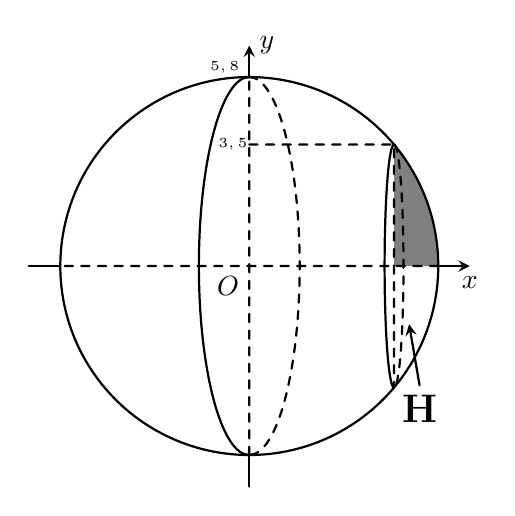
\begin{tikzpicture}[line join=round, line cap=round,>=stealth,thick,rotate=90,scale=0.8]
	% Hình phải
	\def\bk{3}
	\def\bkba{0.15}
	\def\bkbb{0.8}
	\def\ga{-50}
	\def\gb{180-\ga}
	\def\gc{0-\gb}
	\coordinate (O) at (0,0);
	\coordinate (M) at ($(O) + (\ga:\bk)$);
	\coordinate (N) at ($(O) + (\gb:\bk)$);
	\coordinate (I) at ($(M)!0.5!(N)$);
	\coordinate (J) at ($(O)+(M)-(I)$);
	\draw(M) arc (\ga:\gb:\bk);
	\path let \p1=(I),\p2=(M),\n1={scalar(veclen(\x2-\x1,\y2-\y1)/1cm)} in \pgfextra{\xdef\bke{\n1}};
	\fill[gray](M) arc (\ga:-90:\bk)--(I)--cycle;
	\draw(M) arc (\ga:\gc:\bk);
	\draw(M) arc (0:180:\bke cm and \bkba cm);
	\draw[dashed](M) arc (0:-180:\bke cm and \bkba cm);
	\coordinate (P) at ($(O) + (250:0.9*\bk)$);
	\coordinate (Q) at ($(O) + (235:1.1*\bk)$);
	\path(Q) node [below] {\Large\bf H};
	\coordinate (A) at ($(O) + (180:\bk)$);
	\coordinate (B) at ($(O) + (0:\bk)$);
	\coordinate (C) at ($(O) + (-90:\bk)$);
	\coordinate (D) at ($(O) + (90:\bk)$);
	\draw(B) arc (0:180:\bk cm and \bkbb cm);
	\draw[dashed](B) arc (0:-180:\bk cm and \bkbb cm);
	\draw[dashed](J)--(M)--(N) (C)--(D) (A)--(B);
	\draw[->](Q)--(P);
	\draw[->](C)--($(C)-(0,0.5)$)node[below]{$x$};
	\draw[->](B)--($(B)+(0.5,0)$)node[right]{$y$};
	\draw(A)--($(A)-(0.5,0)$) (D)--($(D)+(0,0.5)$);
	\path(O) node[below left]{$O$};
	\path(J) node[left=-3]{\tiny $3,5$};
	\path($(B)+(0.15,0)$)node[left]{\tiny $5,8$};
\end{tikzpicture}
}\\
Thể tích của khối chân đế bằng bao nhiêu centimét khối (không làm tròn kết quả các phép tính trung gian, chỉ làm tròn kết quả cuối cùng đến hàng phần mười)?
\end{ex}
\Closesolutionfile{ans}
\label{mylt}
\centerline{\rule[0.5ex]{2cm}{1pt} HẾT \rule[0.5ex]{2cm}{1pt}}

\newpage
\setcounter{page}{1}
\rfoot{Trang \thepage}
\begin{center}
\bf ĐÁP ÁN PHẦN I
\inputansbox[1]{6}{ansMyLTTN}
\end{center}
\begin{center}
\bf ĐÁP ÁN PHẦN II
\end{center}
\inputansbox[2]{2}{ansMyLTTF}
\begin{center}
\bf ĐÁP ÁN PHẦN III
\end{center}
\inputansbox[3]{3}{ansMyLTSA}
\end{document}